\documentclass{standalone}
\usepackage{tikz}
\begin{document}
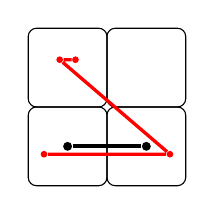
\begin{tikzpicture}[scale=1.0]
  % draw rounded cell boxes
  \draw[rounded corners=3pt] (0,0) rectangle (1,1);
  \draw[rounded corners=3pt] (0,1) rectangle (1,2);
  \draw[rounded corners=3pt] (1,0) rectangle (2,1);
  \draw[rounded corners=3pt] (1,1) rectangle (2,2);
  \node[circle, fill=red, inner sep=0.03cm] (obs4377147776_pt0) at (0.2,0.4) {};
  \node[circle, fill=red, inner sep=0.03cm] (obs4377147776_pt1) at (0.4,1.6) {};
  \node[circle, fill=red, inner sep=0.03cm] (obs4377147776_pt2) at (0.6,1.6) {};
  \node[circle, fill=red, inner sep=0.03cm] (obs4377147776_pt3) at (1.8,0.4) {};
  \draw[red, line width=1.2pt] (obs4377147776_pt0) -- (obs4377147776_pt3) -- (obs4377147776_pt1) -- (obs4377147776_pt2);
  % draw black chords for chord_row_cells
  \node[circle, fill=black, inner sep=0.04cm] (chord_row0_left) at (0.5,0.5) {};
  \node[circle, fill=black, inner sep=0.04cm] (chord_row0_right) at (1.5,0.5) {};
  \draw[black, line width=1.5pt] (chord_row0_left) -- (chord_row0_right);
\end{tikzpicture}
\end{document}